\documentclass[a4paper]{report}

%====================== PACKAGES ======================
\usepackage{xcolor}
\usepackage{indentfirst}
\usepackage{pgfplots}
\pgfplotsset{compat=1.18}
\usepackage{mdframed}
\usepackage{fontawesome5}
\usepackage{titlesec}
\usepackage{lmodern}
\usepackage[french]{babel}
\usepackage{listings}
\usepackage[utf8]{inputenc}
\usepackage{enumitem}
\usepackage{color}
\usepackage{booktabs}
\usepackage{amssymb}

\definecolor{mGreen}{rgb}{0,0.6,0}
\definecolor{mGray}{rgb}{0.5,0.5,0.5}
\definecolor{mPurple}{rgb}{0.58,0,0.82}
\definecolor{backgroundColour}{rgb}{0.95,0.95,0.92}

\lstdefinestyle{PythonStyle}{
    backgroundcolor=\color{backgroundColour},
    commentstyle=\color{mGreen},
    keywordstyle=\color{magenta},
    numberstyle=\tiny\color{mGray},
    stringstyle=\color{mPurple},
    basicstyle=\small\ttfamily,
    breaklines=true,
    captionpos=b,
    keepspaces=true,
    numbers=left,
    numbersep=5pt,
    showspaces=false,
    showstringspaces=false,
    tabsize=2,
    language=Python
}

% Nested list bullets
\setlist[itemize,1]{label=\textbullet}
\setlist[itemize,2]{label=--}

% N+ONE brand colors
\definecolor{noneNavy}{HTML}{003049}
\definecolor{noneOrange}{HTML}{F77F00}
\definecolor{projectorange}{HTML}{F77F00}

% Custom colors
\definecolor{notecolor}{RGB}{230,240,255}
\definecolor{bordercolor}{RGB}{50,100,200}
\definecolor{titlecolor}{RGB}{30,60,120}

\usepackage{tikz}
\usetikzlibrary{arrows.meta,positioning,shapes.geometric}

\usepackage{amsmath}
\usepackage{graphicx}
\usepackage[colorinlistoftodos]{todonotes}
\usepackage{url}
\usepackage[section]{placeins}
\usepackage{hyperref}
\usepackage{acronym}
\usepackage{array}
\usepackage{tabularx}
\usepackage{multirow}
\usepackage[justification=centering]{caption}
\usepackage{setspace}
\usepackage{abstract}
\usepackage[T1]{fontenc}
\usepackage{csquotes}
\usepackage[top=2cm, bottom=2cm, left=2cm, right=2cm]{geometry}
\usepackage{subfig}
\usepackage{subcaption}
\usepackage{eurosym}

% ==== Encadrés ====
\usepackage[most]{tcolorbox}
\tcbset{
  colframe=noneOrange,
  colback=white,
  coltitle=black,
  boxrule=0.8pt,
  arc=3pt,
  left=6pt, right=6pt, top=6pt, bottom=6pt
}

%====================== METADATA ======================
\setcounter{secnumdepth}{4}
\setcounter{tocdepth}{4}

\hypersetup{
  pdfauthor  = {MADANI Anas},
  pdftitle   = {Rapport de Stage 2A},
  pdfsubject = {Développement d'une Application Web Sécurisée pour la Gestion des Appels d'Offres},
  pdfkeywords = {Django, React, JWT, RBAC, AES-256-GCM, Docker, GitHub Actions},
  pdfstartview = {FitH}
}

%======================== DOCUMENT ========================
\begin{document}
\onehalfspacing
\selectlanguage{french}
\newcommand{\HRule}{\rule{\linewidth}{0.5mm}}
\renewcommand{\arraystretch}{1.5}

%---------- Page de garde ----------
\begin{titlepage}
\begin{center}

  % Logos
  \begin{minipage}{0.45\textwidth}
    \begin{flushleft}
      
\includegraphics[scale=0.4]{ensias.png}
    \end{flushleft}
  \end{minipage}
  \begin{minipage}{0.48\textwidth}
    \begin{flushright}
      % TODO: Remplacer par le logo N+ONE quand disponible
      % \includegraphics[height=1.8cm]{images/nplus1_logo.png}

      \includegraphics[width=0.7\textwidth]{/home/an2s/Documents/Stage_2A/rapport/logos/nplusone.png}
    \end{flushright}
  \end{minipage}

  \vspace*{.06\textheight}

  \textsc{\Large École Nationale Supérieure d'Informatique et d'Analyse des Systèmes -- RABAT}\\[1.5cm]
  \textsc{\huge \bfseries Rapport de Stage de 2\textsuperscript{ème} Année}\\[0.5cm]
  \textsc{\large Filière Génie Logiciel}\\[1cm]

  \HRule \\[0.4cm]
  {\huge \bfseries Développement d'une Application Web Sécurisée\\[0.3cm]
  pour la Gestion des Appels d'Offres}\\[0.4cm]
  \HRule \\[0.5cm]

  \begin{center}
    {\large Réalisé au sein de : \textbf{N+ONE DATACENTERS, Casablanca}}\\[0.3cm]
    {\large Période : \textbf{06 août -- 06 septembre 2025}}
  \end{center}

  \vspace{0.8cm}

  \begin{minipage}{0.4\textwidth}
    \begin{flushleft}\large
      \emph{Réalisé par :}\\[0.5cm]
      Anas \textsc{Madani}
    \end{flushleft}
  \end{minipage}
  \begin{minipage}{0.5\textwidth}
    \begin{flushright}\large
      \emph{Encadré par :}\\[0.3cm]
      M. Ayoub \textsc{Amellaln} \textsc{(N+ONE)}\\
      M. Amine \textsc{El Mahi} \textsc{(N+ONE)}
      % TODO: Ajouter encadrant académique ENSIAS si applicable
    \end{flushright}
  \end{minipage}

  \vfill
  {\large Année universitaire 2024/2025}

\end{center}
\end{titlepage}


%---------- Page blanche ----------
\newpage
~
\thispagestyle{empty}
\newpage

%---------- Dédicace + Remerciements + Résumé + Abréviations ----------
\newgeometry{top=3cm, bottom=3cm, left=3cm, right=3cm}
\begin{titlepage}
  \begin{center}
    \vspace*{4cm}
    {\Huge \textbf{Dédicace}}

    \vspace{2cm}

    \begin{minipage}{0.85\textwidth}
      \onehalfspacing

      \textbf{À ma mère.}  
      Ton amour, ta patience et ta confiance m’ont accompagné à chaque étape de ce travail.  
      Tu as toujours été ma source de tendresse et de force.  
      Que Dieu te protège et t’accorde santé, paix et longue vie.

      \vspace{0.3cm}

      \textbf{À mon père.}  
      Ton sens du devoir, ta discrétion et ta présence solide m’ont transmis la rigueur et le courage.  
      Merci pour tous tes sacrifices.  
      Que Dieu te préserve et t’accorde une vie paisible et épanouie.

      \vspace{0.3cm}

      \textbf{À mes frères et à ma sœur.}  
      Vous êtes bien plus qu’une famille : vous êtes mes repères et mes complices.  
      Merci pour votre affection, vos encouragements et votre confiance sans faille.

      \vspace{0.3cm}

      \textbf{À mon oncle Idriss.}  
      Pour ta gentillesse, tes conseils et ta présence. Merci d’avoir cru en moi.

      \vspace{0.3cm}

      \textbf{À ma famille et à mes amis proches.}  
      Merci pour votre soutien constant, vos mots réconfortants et votre bienveillance.  
      Chacun de vous, à sa manière, a contribué à ce projet.

      \vspace{0.8cm}

      \begin{flushright}
        Anas
      \end{flushright}
    \end{minipage}
  \end{center}\end{titlepage}
\restoregeometry

%---------- Remerciements ----------

\begin{figure}[!h]
\begin{center}
\vspace{1.5cm}

\includegraphics[height=1.8cm]{presentation/remerci.png}
\end{center}
\end{figure}
\vspace{0.5cm}

\begin{center}
    \LARGE \textbf{Remerciements}
\end{center}

\vspace{1cm}

\begin{onehalfspacing}

Je tiens d’abord à remercier mes encadrants chez \textbf{N+ONE DATACENTERS}, 
\textbf{M. Ayoub Amellaln} et \textbf{M. Amine El Mahi}, pour leur confiance, 
leur disponibilité et leurs conseils tout au long de ce stage. 
Merci de m’avoir guidé simplement et avec bienveillance, et de m’avoir offert 
un cadre de travail agréable et motivant.

\vspace{0.5cm}

Je remercie aussi le corps enseignant de l’\textbf{ENSIAS} pour la formation 
solide qu’il m’a donnée pendant ces deux ans, 
et tout particulièrement les enseignants de la filière Génie Logiciel.

\vspace{0.5cm}

Enfin, merci à toute l’équipe de \textbf{N+ONE DATACENTERS} pour leur accueil chaleureux 
et pour avoir rendu mon intégration facile dès le premier jour.

\end{onehalfspacing}\vspace{0.3cm}
}
\end{spacing}

\begin{figure}[!h]
\begin{center}
\vspace{1cm}

\includegraphics[height=1cm]{presentation/remerc2.png}
\end{center}
\end{figure}

\newpage

%---------- Résumé ----------

%---------- Résumé ----------

\hskip7mm
\vspace{3cm}
\begin{center}
{\textbf{\Huge Résumé}}
\end{center}
\vspace{1cm}

\begin{spacing}{1.15}

{\large
Ce rapport présente le développement d'une application web sécurisée de gestion
des appels d'offres, réalisé lors d'un stage d'un mois au sein de \textbf{N+ONE DATACENTERS}
à Casablanca. Le projet répond à un besoin concret : remplacer un processus fragmenté
(emails, Excel, partages réseau) par une solution centralisée, traçable et sécurisée.
}
\vspace{0.4cm}

{\large
L'application repose sur une architecture monolithe modulaire (\textbf{Django REST Framework}
côté backend, \textbf{React.js} côté frontend) déployée via \textbf{Docker Compose}
avec un proxy Nginx en HTTPS. Elle couvre l'intégralité du cycle de vie d'un appel
d'offres : de la création au brouillon jusqu'à l'attribution du marché, en passant
par la publication, la collecte des soumissions et l'évaluation des candidats.
}
\vspace{0.4cm}

{\large
Les principales fonctionnalités de sécurité implémentées sont :
l'authentification \textbf{JWT} avec access token en mémoire et refresh token en cookie
\texttt{httpOnly} scopé, le contrôle d'accès basé sur les rôles (\textbf{RBAC}) à quatre
niveaux (ADMIN, MANAGER, ANALYST, VIEWER), le chiffrement sélectif
\textbf{AES-256-GCM} des documents sensibles, et un journal d'audit complet.
Un portail public isolé permet aux sociétés externes de déposer leurs propositions
sans compte utilisateur, avec rate limiting et vérification des deadlines côté serveur.
}
\vspace{0.4cm}

{\large
Un pipeline d'intégration continue (GitHub Actions) exécute automatiquement
les tests pytest et le lint flake8 à chaque push. L'application est déployable
en une commande (\texttt{docker-compose up}).
}
\vspace{0.8cm}

\noindent\rule{\linewidth}{0.4pt}
\vspace{0.3cm}

\noindent
{\large \textbf{Mots-clés :} Appels d'offres, Django REST Framework, React.js,
JWT, RBAC, AES-256-GCM, Docker Compose, GitHub Actions, Portail public, Audit.}

\end{spacing}

\newpage
%---------- Abstract ----------

\hskip7mm
\vspace{3cm}
\begin{center}
{\textbf{\Huge Abstract}}
\end{center}
\vspace{1cm}

\begin{spacing}{1.15}
{\large
This report presents the development of a secure web application for procurement
management, carried out during a one-month internship at \textbf{N+ONE DATACENTERS}
in Casablanca. The project addresses a concrete need: replacing a fragmented process
(emails, Excel, shared drives) with a centralized, traceable, and secure solution.

\vspace{0.4cm}

The application is built on a modular monolith architecture (\textbf{Django REST Framework}
backend, \textbf{React.js} frontend) deployed via \textbf{Docker Compose} with an Nginx
HTTPS proxy. It covers the complete procurement lifecycle: from draft creation to contract
award, through publication, submission collection, and candidate evaluation.

\vspace{0.4cm}

The main security features implemented are: \textbf{JWT authentication} with access token
in memory and refresh token in a scoped \texttt{httpOnly} cookie, four-level
\textbf{role-based access control} (RBAC), selective \textbf{AES-256-GCM encryption}
of sensitive documents, and a comprehensive audit log. An isolated public portal allows
external companies to submit proposals without an account, with IP-based rate limiting
and server-side deadline enforcement.

\vspace{0.4cm}

A continuous integration pipeline (GitHub Actions) automatically runs pytest tests and
flake8 lint on every push. The application deploys in a single command
(\texttt{docker-compose up}).

\vspace{0.8cm}

\noindent\rule{\linewidth}{0.4pt}
\vspace{0.3cm}

\noindent\textbf{Keywords:} Procurement management, Django REST Framework, React.js,
JWT, RBAC, AES-256-GCM, Docker Compose, GitHub Actions, Public portal, Audit log.
}
\end{spacing}

\newpage

%---------- Liste des abréviations ----------

\chapter*{Liste des abréviations}
\addcontentsline{toc}{chapter}{Liste des abréviations}

\begin{acronym}[AES-256-GCM]
  \acro{AES}{Advanced Encryption Standard}
  \acro{API}{Application Programming Interface}
  \acro{CI}{Continuous Integration}
  \acro{CORS}{Cross-Origin Resource Sharing}
  \acro{CRUD}{Create, Read, Update, Delete}
  \acro{DRF}{Django REST Framework}
  \acro{GCM}{Galois/Counter Mode}
  \acro{HTTP}{HyperText Transfer Protocol}
  \acro{HTTPS}{HyperText Transfer Protocol Secure}
  \acro{JWT}{JSON Web Token}
  \acro{MIME}{Multipurpose Internet Mail Extensions}
  \acro{ORM}{Object-Relational Mapper}
  \acro{PDF}{Portable Document Format}
  \acro{RBAC}{Role-Based Access Control}
  \acro{REST}{Representational State Transfer}
  \acro{SPA}{Single Page Application}
  \acro{SQL}{Structured Query Language}
  \acro{TLS}{Transport Layer Security}
  \acro{UUID}{Universally Unique Identifier}
  \acro{XSS}{Cross-Site Scripting}
\end{acronym}

\newpage


%---------- Tables ----------
\tableofcontents

\listoffigures
\addcontentsline{toc}{chapter}{Liste des figures}
\thispagestyle{empty}
\newpage

\listoftables
\addcontentsline{toc}{chapter}{Liste des tableaux}
\newpage

%---------- Corps ----------
~
\thispagestyle{empty}
\setcounter{page}{0}
\newpage

\chapter*{Introduction Générale}
\addcontentsline{toc}{chapter}{Introduction Générale}
\markboth{Introduction Générale}{Introduction Générale}

\begin{spacing}{1.25}
{\large

Dans un contexte économique où la commande publique et les marchés d'entreprise
représentent des volumes financiers considérables, la gestion rigoureuse des appels
d'offres constitue un enjeu stratégique majeur. Pour les organisations qui publient
et évaluent régulièrement ces appels, la qualité du processus détermine directement
la compétitivité, la conformité réglementaire et la maîtrise des délais.

\todo[inline, color=orange!30]{À COMPLÉTER : contexte spécifique N+ONE — secteur datacenter, volume d'appels d'offres, positionnement marché}

\section*{Contexte du stage}

Ce stage de deuxième année a été effectué au sein de \textbf{N+ONE DATACENTERS},
société spécialisée dans l'hébergement et la gestion d'infrastructure datacenter,
basée à Casablanca, au Maroc. D'une durée d'un mois, du 6 août au 6 septembre 2025,
il s'inscrit dans le cadre de la formation en Génie Logiciel à l'École Nationale
Supérieure d'Informatique et d'Analyse des Systèmes (ENSIAS) de Rabat.

\todo[inline, color=orange!30]{À COMPLÉTER : description activité N+ONE, nombre d'employés, nombre de datacenters, clients types}

\section*{Problématique}

Avant ce projet, la gestion des appels d'offres chez N+ONE reposait sur des outils
non spécialisés : échanges par email, suivi sous tableurs Excel et stockage de documents
sur disques partagés. Cette approche fragmentée engendrait plusieurs problèmes
opérationnels :

\begin{itemize}
    \item \textbf{Absence de centralisation} : les informations étaient dispersées
    entre boîtes mail, fichiers Excel et répertoires réseau, rendant le suivi global
    impossible sans consolidation manuelle.

    \item \textbf{Risque de dépassement de délais} : aucun mécanisme d'alerte automatique
    ne prévenait les responsables à l'approche des dates limites de soumission
    ou d'évaluation.

    \item \textbf{Sécurité insuffisante} : les offres financières (données sensibles)
    circulaient par email ou étaient stockées en clair sur des partages réseau,
    sans chiffrement ni contrôle d'accès granulaire.

    \item \textbf{Traçabilité absente} : aucun historique ne permettait de savoir
    qui avait modifié quoi, ni quand, compromettant la conformité et la gouvernance.

    \item \textbf{Surcharge avant les échéances} : la réception de plusieurs soumissions
    simultanées en fin de période créait un goulot d'étranglement,
    les agents devant saisir manuellement les informations des candidats.
\end{itemize}

\section*{Objectifs du stage}

L'objectif principal était de concevoir et développer une \textbf{application web
sécurisée de gestion des appels d'offres}, couvrant l'intégralité du cycle de vie :
de la création de l'offre jusqu'à l'attribution du marché, en passant par la publication,
la collecte des soumissions et l'évaluation des candidats.

Les objectifs techniques et fonctionnels définis en début de stage étaient les suivants :

\begin{enumerate}
    \item Authentification sécurisée avec gestion des rôles (RBAC) ;
    \item Cycle de vie complet des appels d'offres avec transitions d'état contrôlées ;
    \item Portail public permettant aux sociétés externes de déposer leurs offres
    sans compte utilisateur ;
    \item Chiffrement AES-256-GCM des documents financiers sensibles ;
    \item Notifications automatiques (délais, changements de statut) ;
    \item Génération de rapports PDF ;
    \item Journal d'audit traçant toutes les actions sur les ressources ;
    \item Déploiement Dockerisé reproductible avec pipeline CI/CD.
\end{enumerate}

\section*{Plan du rapport}

Ce rapport s'organise en trois parties principales.

La \textbf{Partie 1} présente le cahier des charges : après une introduction à
l'organisme d'accueil et au domaine des appels d'offres, elle détaille l'analyse
des besoins fonctionnels et non-fonctionnels, l'étude des solutions existantes
et la justification du développement sur mesure.

La \textbf{Partie 2} couvre l'analyse, la conception et l'architecture : choix
technologiques argumentés, planification, modélisation UML (cas d'utilisation,
diagrammes d'activité, séquences) et conception détaillée du système (modèle de
données, API REST, architecture de sécurité).

La \textbf{Partie 3} décrit la réalisation et la mise en œuvre : implémentation
des modules backend et frontend, présentation des interfaces, et résultats
des tests de validation.

}
\end{spacing}

\newpage

\chapter{Cahier des Charges}

\begin{spacing}{1.25}
{\large

\section{Présentation de l'organisme d'accueil}

\subsection{N+ONE DATACENTERS}

\todo[inline, color=orange!30]{À RÉDIGER : Présentation N+ONE DATACENTERS — date de création, siège social (Casablanca), activité principale (hébergement/gestion datacenter), nombre de datacenters et capacité, clients types (entreprises, opérateurs, administrations), effectif approximatif, certifications (ISO 27001, Tier III ?)}

\subsection{Environnement de travail}

\todo[inline, color=orange!30]{À COMPLÉTER : décrire l'équipe, le département d'accueil, les outils utilisés en interne}

Le stage s'est déroulé au sein du département \textit{\colorbox{yellow}{[NOM DU DÉPARTEMENT]}},
sous la supervision de M. Ayoub \textsc{Amellaln} et M. Amine \textsc{El Mahi}.

\begin{figure}[ht]
\centering
\fbox{%
  \begin{minipage}{0.85\textwidth}
    \vspace{2cm}
    \centering
    \textit{[À INSÉRER — Organigramme de N+ONE DATACENTERS — images/organigramme.png]}
    \vspace{2cm}
  \end{minipage}%
}
\caption{Organigramme de N+ONE DATACENTERS}
\label{fig:organigramme}
\end{figure}

% -------------------------------------------------------------------

\section{Présentation du sujet}

\subsection{Les appels d'offres}

Un appel d'offres est une procédure formalisée par laquelle une organisation (le
\textit{maître d'ouvrage}) invite des fournisseurs ou prestataires potentiels à
soumettre des propositions commerciales et techniques pour la réalisation d'un marché.
Cette procédure garantit la mise en concurrence, la transparence et la traçabilité
des décisions d'achat.

Le cycle de vie d'un appel d'offres se décompose en plusieurs phases distinctes,
illustrées dans la figure~\ref{fig:lifecycle} :

\begin{enumerate}
    \item \textbf{BROUILLON (DRAFT)} : l'offre est en cours de rédaction,
    non visible par les candidats.
    \item \textbf{PUBLIÉE (PUBLISHED)} : l'offre est ouverte, les sociétés
    externes peuvent soumettre leurs propositions via le portail public.
    \item \textbf{ÉVALUATION} : la date limite de soumission est passée ;
    les responsables évaluent et scorent les candidatures reçues.
    \item \textbf{ATTRIBUÉE (AWARDED)} : le marché est attribué au candidat retenu.
    \item \textbf{ANNULÉE (CANCELLED)} : l'offre est interrompue à tout moment
    avant attribution.
\end{enumerate}

\begin{figure}[ht]
\centering
\fbox{%
  \begin{minipage}{0.85\textwidth}
    \vspace{2cm}
    \centering
    \textit{[À INSÉRER — Cycle de vie d'un appel d'offres — images/lifecycle.png]}
    \vspace{2cm}
  \end{minipage}%
}
\caption{Cycle de vie d'un appel d'offres}
\label{fig:lifecycle}
\end{figure}

\subsection{Les acteurs du système}

Le système distingue deux catégories d'utilisateurs :

\paragraph{Acteurs internes} Membres du personnel de N+ONE disposant d'un compte
applicatif, répartis en quatre rôles :

\begin{itemize}
    \item \textbf{ADMIN} : administrateur système, gère les comptes utilisateurs
    et accède au journal d'audit complet.
    \item \textbf{MANAGER} : responsable d'offres, crée et pilote les appels d'offres,
    attribue les marchés, génère les rapports PDF.
    \item \textbf{ANALYST} : évaluateur, score les soumissions et consulte
    les dossiers des candidats.
    \item \textbf{VIEWER} : lecteur seul, consulte les offres publiées
    sans pouvoir modifier quoi que ce soit.
\end{itemize}

\paragraph{Acteurs externes} Sociétés soumissionnaires accédant uniquement au
portail public sans créer de compte. Elles peuvent consulter les offres ouvertes
et déposer leurs propositions directement en ligne.

% -------------------------------------------------------------------

\section{Analyse des besoins}

\subsection{Besoins fonctionnels}

\begin{table}[ht]
\centering
\caption{Besoins fonctionnels du système}
\label{tab:besoins-fonctionnels}
\begin{tabularx}{\textwidth}{|l|X|}
\hline
\textbf{Module} & \textbf{Description} \\
\hline
Authentification & Connexion sécurisée, déconnexion, rafraîchissement de session \\
\hline
Gestion des offres & Création, modification, publication, transition de statut, annulation \\
\hline
Candidats et soumissions & Enregistrement des candidats, dépôt de soumissions, scoring technique et financier \\
\hline
Documents & Upload multipart, téléchargement sécurisé, chiffrement sélectif \\
\hline
Portail public & Consultation des offres publiées et dépôt de soumissions sans authentification \\
\hline
Notifications & Alertes automatiques : délais approchants, changements de statut, attribution \\
\hline
Rapports & Export PDF d'une offre (synthèse, tableau des scores, candidat retenu) \\
\hline
Audit & Journal des actions sur toutes les ressources (qui, quoi, quand, depuis où) \\
\hline
Administration & Gestion des comptes utilisateurs (création, désactivation, changement de rôle) \\
\hline
\end{tabularx}
\end{table}

\subsection{Besoins non-fonctionnels}

\begin{description}
    \item[Sécurité] Authentification par JWT (token en mémoire, cookie httpOnly),
    contrôle d'accès basé sur les rôles (RBAC), chiffrement AES-256-GCM des documents
    sensibles, audit complet, protection contre les injections SQL, HTTPS obligatoire.

    \item[Performance] Réponses API inférieures à 500 ms pour les listes paginées.
    Pagination côté serveur (20 offres par page). Chiffrement uniquement sur les
    documents marqués sensibles pour ne pas pénaliser les uploads standards.

    \item[Disponibilité] Redémarrage automatique des conteneurs Docker en cas d'échec
    (\texttt{restart: unless-stopped}). Vérifications de santé (\textit{health checks})
    sur chaque service.

    \item[Traçabilité] Toute action d'écriture (création, modification, téléchargement,
    export, connexion) est enregistrée dans le journal d'audit avec l'adresse IP,
    l'utilisateur et le contenu des modifications.

    \item[Maintenabilité] Architecture modulaire (8 applications Django indépendantes),
    pipeline CI automatique (tests + lint à chaque push), structure de projet
    documentée.

    \item[Reproductibilité] Déploiement en une commande (\texttt{docker-compose up}).
    Variables d'environnement pour tous les secrets, aucune valeur en dur dans le code.
\end{description}

% -------------------------------------------------------------------

\section{Évaluation et justification de la solution}

\subsection{Étude de l'existant}

Plusieurs solutions existent sur le marché pour la gestion des appels d'offres :

\begin{table}[ht]
\centering
\caption{Comparaison des solutions existantes}
\label{tab:existant}
\begin{tabularx}{\textwidth}{|l|X|X|X|}
\hline
\textbf{Solution} & \textbf{Points forts} & \textbf{Limites} & \textbf{Adapté ?} \\
\hline
SAP Ariba & Complète, intégration ERP & Coût élevé (licences), délai de déploiement long, sur-mesure impossible & Non \\
\hline
Proactis & Gestion marchés publics & Coût prohibitif pour une PME, rigidité du workflow & Non \\
\hline
OpenProposal / open source & Gratuit & Documentation insuffisante, peu maintenu, pas de support & Non \\
\hline
Excel + partage réseau & Gratuit, familier & Non sécurisé, non traçable, fragile, pas de portail externe & Non \\
\hline
\textbf{Développement sur mesure} & \textbf{Adapté exactement aux besoins} & Délai de développement & \textbf{Oui} \\
\hline
\end{tabularx}
\end{table}

\subsection{Critique de l'existant}

Aucune des solutions commerciales n'est adaptée au contexte de ce stage pour
trois raisons cumulatives. D'abord, le \textbf{budget nul} interdit les licences SaaS.
Ensuite, le \textbf{délai d'un mois} exclut tout déploiement et personnalisation
de produit tiers. Enfin, le besoin d'un \textbf{chiffrement sélectif} des documents
financiers et d'un portail public isolé dépasse les fonctionnalités standard
des outils génériques.

La solution Excel actuelle, bien que pratique, expose l'entreprise à des risques
réels : perte de données, accès non contrôlé aux offres financières, impossibilité
de retrouver l'historique des modifications.

\subsection{Justification du développement sur mesure}

Le développement d'une application web sur mesure est la seule option répondant
simultanément à toutes les contraintes :

\begin{itemize}
    \item Workflow exact du processus N+ONE (statuts, rôles, notifications) ;
    \item Chiffrement AES-256-GCM intégré nativement ;
    \item Portail public isolé pour les sociétés externes ;
    \item Coût nul en licences (stack open source) ;
    \item Déployable sur l'infrastructure existante de N+ONE.
\end{itemize}

\paragraph{Estimation des coûts d'infrastructure} En cas de déploiement en production,
le coût se limiterait à l'infrastructure serveur : environ 50 à 100 \euro/mois
sur un serveur cloud (ou nul si déployé sur les serveurs internes N+ONE), contre
plusieurs milliers d'euros annuels pour une licence SAP Ariba.


}
\end{spacing}

\newpage

\chapter{Analyse, Conception et Architecture}

\begin{spacing}{1.25}
{\large

\section{Choix technologiques}

Le choix de la stack technique a été guidé par trois critères : la rapidité de
développement (délai d'un mois), la maturité des outils (documentation, communauté)
et la sécurité intégrée (pas d'add-ons nécessaires pour les fonctionnalités critiques).

\begin{table}[ht]
\centering
\caption{Comparaison et justification des choix technologiques}
\label{tab:techstack}
\begin{tabularx}{\textwidth}{|l|l|X|}
\hline
\textbf{Couche} & \textbf{Choix retenu} & \textbf{Justification dans le contexte du stage} \\
\hline
Backend & Django + DRF & Stack maîtrisée. L'administration Django et les modules DRF (sérialisation, permissions, pagination) évitent de réimplémenter des fonctionnalités standard, ce qui est décisif sur un délai d'un mois. \\
\hline
Frontend & React.js + Vite & Framework connu, documentation abondante, large choix de composants UI. Le choix est pragmatique : utiliser ce qu'on maîtrise plutôt que d'apprendre un nouveau framework en parallèle du développement. \\
\hline
Base de données & PostgreSQL & Standard de facto avec Django. Support natif du type JSON (utile pour \texttt{AuditLog.changes}) et de \texttt{TIMESTAMPTZ} pour la gestion précise des deadlines. \\
\hline
Authentification & JWT (simplejwt) & Bibliothèque officielle de l'écosystème DRF, intégrable en quelques heures. La solution couvre le besoin (usage interne, une seule organisation) sans nécessiter un serveur OAuth2 dédié, hors scope pour ce stage. \\
\hline
Conteneurisation & Docker Compose & Outil maîtrisé permettant de démarrer les 5 services en une commande. Kubernetes serait pertinent pour un déploiement en production à grande échelle, mais constitue une complexité opérationnelle injustifiée ici. \\
\hline
Proxy & Nginx + HTTPS & Configuration TLS simple et bien documentée. Gunicorn seul ne gère pas le TLS nativement et n'est pas conçu pour être exposé directement. \\
\hline
CI/CD & GitHub Actions & CI gratuite, intégrée au dépôt, sans infrastructure à maintenir. Adapté à un projet solo avec un seul environnement cible. \\
\hline
\end{tabularx}
\end{table}

\paragraph{Django} a été préféré pour son administration intégrée (économie de 3 à 4
jours), son ORM prévenant nativement les injections SQL, et DRF qui fournit
sérialisation, permissions et pagination sans code supplémentaire.

\paragraph{PostgreSQL} offre un support natif des colonnes JSON (utile pour
\texttt{AuditLog.changes}), un type \texttt{TIMESTAMPTZ} précis pour le suivi des
délais, et de meilleures performances sur la recherche textuelle avec l'opérateur
\texttt{ILIKE}.

\paragraph{Docker Compose} permet de démarrer l'ensemble du système (frontend,
backend, base de données, proxy, scheduler) en une seule commande,
garantissant la reproductibilité entre environnements de développement
et de démonstration.

% -------------------------------------------------------------------

\section{Conduite du projet}

\subsection{Méthodologie adoptée}

Face à une contrainte de délai d'un mois et à un périmètre fonctionnel
initialement estimé mais susceptible d'être affiné au fil des retours,
une approche \textbf{Agile adaptée} a été adoptée, s'inspirant du cadre
Scrum tout en tenant compte du contexte d'un développeur solo.

Chaque semaine constituait un sprint d'une durée fixe, avec un livrable
démontrable à la fin. En début de sprint, le backlog était revu et priorisé
en concertation avec les encadrants ; en fin de sprint, une démo informelle
permettait de valider les fonctionnalités réalisées et d'ajuster les priorités
pour le sprint suivant. Le suivi quotidien des tâches a été assuré via un
tableau Kanban personnel organisé en trois colonnes : \textit{À faire},
\textit{En cours}, \textit{Terminé}.

Ce choix a été préféré à une approche cycle en V classique pour deux raisons
principales : la nature incrémentale du projet (chaque sprint livrait une
couche fonctionnelle complète et testable), et la nécessité de faire valider
les choix de sécurité au fur et à mesure plutôt qu'en fin de projet.

% -------------------------------------------------------------------

\subsection{Planification et backlog}

\subsubsection{Backlog produit}

Les fonctionnalités ont été priorisées selon le modèle \textbf{MoSCoW}
(Must-Have, Should-Have, Could-Have), en accord avec les exigences
exprimées par les encadrants en début de stage.

\begin{table}[ht]
\centering
\caption{Backlog produit}
\label{tab:backlog}
\begin{tabularx}{\textwidth}{|l|l|X|c|c|}
\hline
\textbf{ID} & \textbf{Priorité} & \textbf{User Story} & \textbf{Sprint} & \textbf{Statut} \\
\hline
US-01 & Haute & Admin peut créer et gérer les comptes utilisateurs avec rôles & S1 & \checkmark \\
\hline
US-02 & Haute & Utilisateur se connecte via email/mot de passe, reçoit un JWT & S1 & \checkmark \\
\hline
US-03 & Haute & Access token rafraîchi automatiquement via cookie httpOnly & S1 & \checkmark \\
\hline
US-04 & Haute & Manager peut créer un appel d'offres (titre, budget, délais) & S2 & \checkmark \\
\hline
US-05 & Haute & Manager peut publier, clôturer ou attribuer une offre & S2 & \checkmark \\
\hline
US-06 & Moyenne & Analyst peut consulter toutes les offres et évaluer les soumissions & S2 & \checkmark \\
\hline
US-07 & Moyenne & Upload de documents PDF/DOCX associés à une offre & S2 & \checkmark \\
\hline
US-08 & Haute & Contrôle d'accès RBAC appliqué sur tous les endpoints & S3 & \checkmark \\
\hline
US-09 & Haute & Documents financiers chiffrés AES-256-GCM à l'upload & S3 & \checkmark \\
\hline
US-10 & Haute & Journal d'audit enregistrant toutes les opérations d'écriture & S3 & \checkmark \\
\hline
US-11 & Moyenne & Notifications automatiques générées avant expiration des délais & S3 & \checkmark \\
\hline
US-12 & Haute & Société externe soumet une offre via portail public sans compte & S4 & \checkmark \\
\hline
US-13 & Moyenne & Export PDF d'un rapport de synthèse par offre & S4 & \checkmark \\
\hline
US-14 & Moyenne & Pipeline CI (lint flake8 + pytest) déclenché à chaque push & S4 & \checkmark \\
\hline
\end{tabularx}
\end{table}

\subsubsection{Diagramme de Gantt}

\begin{figure}[ht]
\centering
\fbox{%
  \begin{minipage}{0.92\textwidth}
    \vspace{3.5cm}
    \centering
    \textit{[Diagramme de Gantt -- à insérer]}
    \vspace{3.5cm}
  \end{minipage}%
}
\caption{Diagramme de Gantt du projet (6 août -- 6 septembre 2025)}
\label{fig:gantt}
\end{figure}

% -------------------------------------------------------------------

\subsection{Déroulement des sprints}

Le projet a été découpé en quatre sprints hebdomadaires, chacun centré sur un
objectif livrable.

\begin{description}
    \item[Sprint 1 (6--12 août)] Fondations : Docker Compose, Django, PostgreSQL,
    authentification JWT, modèle User avec rôles.
    Livrable : connexion fonctionnelle, endpoints auth testés via Postman.

    \item[Sprint 2 (13--19 août)] Fonctionnalités métier : offres, candidats,
    soumissions, frontend React connecté à l'API, upload de documents.
    Livrable : un manager peut créer une offre, enregistrer des soumissions.

    \item[Sprint 3 (20--26 août)] Sécurité et notifications : RBAC, journal d'audit,
    monitoring des délais, chiffrement AES-256-GCM, notifications en application.
    Livrable : rôles appliqués, documents sensibles chiffrés, alertes actives.

    \item[Sprint 4 (27 août -- 6 septembre)] Portail public, rapports PDF,
    tests, pipeline CI, documentation.
    Livrable : application complète, testée, déployable en une commande.
\end{description}

\subsubsection{Bilan des sprints}

\textbf{Sprint 1.} La configuration du réseau Docker (communication inter-conteneurs,
variables d'environnement) a pris plus de temps qu'estimé. La configuration du
cookie httpOnly pour le refresh token a nécessité une phase de recherche sur
la gestion des cookies cross-origin avec DRF. Le livrable a été atteint avec
un jour de retard, récupéré en début de Sprint 2.

\textbf{Sprint 2.} La complexité de l'upload de documents (validation MIME,
gestion des fichiers Django) a conduit à différer le chiffrement AES au Sprint 3,
où il a été intégré naturellement avec les autres fonctionnalités de sécurité.
Les fonctionnalités métier principales ont été livrées dans les délais.

\textbf{Sprint 3.} L'intégration d'AES-256-GCM a nécessité une journée de
recherche non planifiée sur la bibliothèque \texttt{cryptography} (gestion
du nonce, format de stockage). Le scheduler de monitoring des délais a été
simplifié : une boucle shell dans un conteneur dédié plutôt qu'une intégration
Celery, jugée trop complexe pour le délai disponible.

\textbf{Sprint 4.} La configuration du pipeline GitHub Actions (base PostgreSQL
de test, variables d'environnement CI) a été le dernier élément ajouté,
achevé dans les deux derniers jours du stage. La documentation et le script
de démonstration \texttt{seed\_demo.py} ont été finalisés en parallèle.

% -------------------------------------------------------------------

\subsection{Gestion des risques}

\begin{table}[ht]
\centering
\caption{Registre des risques du projet}
\label{tab:risques}
\begin{tabularx}{\textwidth}{|X|c|c|p{5cm}|}
\hline
\textbf{Risque} & \textbf{Probabilité} & \textbf{Impact} & \textbf{Stratégie de mitigation} \\
\hline
Mauvaise estimation de la durée d'une fonctionnalité complexe
& Moyenne & Élevé
& Timeboxing strict de 2 jours par sous-tâche ; descope vers le sprint suivant si dépassé \\
\hline
Instabilité d'une bibliothèque tierce (ex. simplejwt, cryptography)
& Faible & Moyen
& Vérification des versions LTS et activité des dépôts avant adoption \\
\hline
Perte du code source (panne matérielle, suppression accidentelle)
& Faible & Critique
& Dépôt Git privé avec push quotidien, branches de sauvegarde hebdomadaires \\
\hline
Évolution du périmètre fonctionnel en cours de sprint
& Moyenne & Moyen
& Validation du backlog avec le maître de stage en début de chaque sprint \\
\hline
Incompatibilité entre services Docker (version PostgreSQL, réseau)
& Faible & Élevé
& Tests d'intégration dès le Sprint 1 ; health checks sur tous les services \\
\hline
\end{tabularx}
\end{table}


% -------------------------------------------------------------------

\section{Modélisation des besoins}

\subsection{Diagramme de cas d'utilisation}

\begin{figure}[ht]
\centering
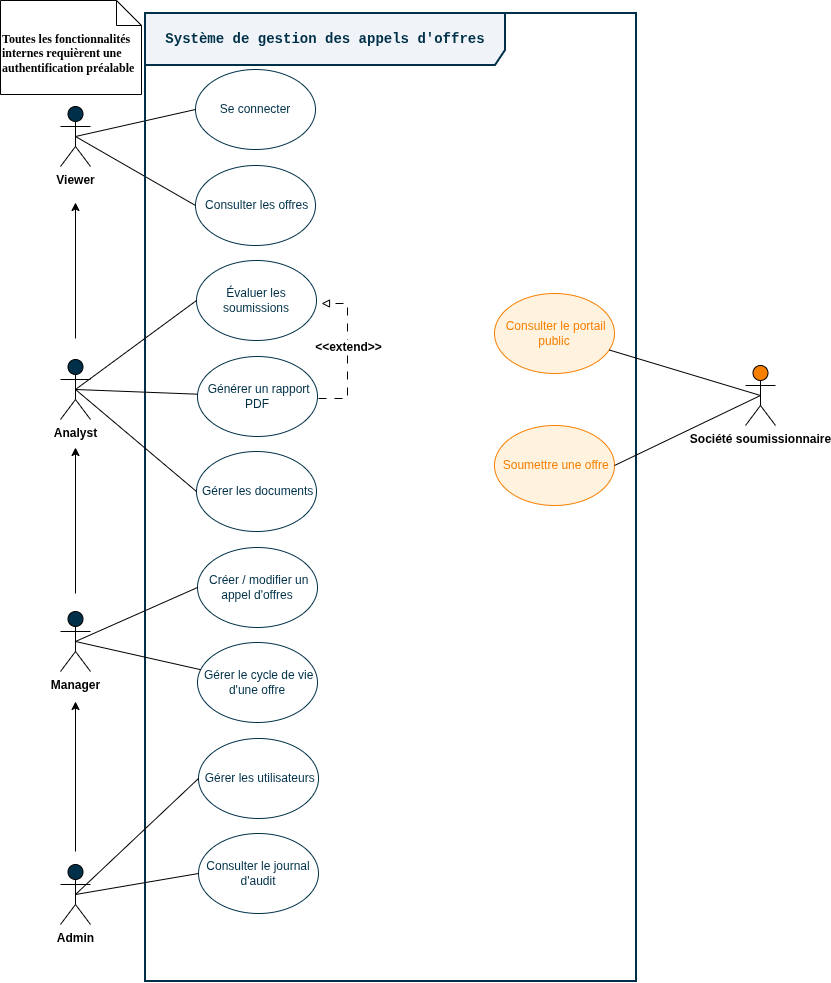
\includegraphics[width=0.9\textwidth]{images/use_case.png}
\caption{Diagramme de cas d'utilisation}
\label{fig:usecase}
\end{figure}

Le diagramme de cas d'utilisation (figure~\ref{fig:usecase}) présente les interactions
entre les cinq acteurs du système et les fonctionnalités exposées.
Les acteurs internes (Admin, Manager, Analyst, Viewer) s'authentifient via JWT.
L'acteur externe (Société soumissionnaire) accède uniquement au portail public
sans authentification.

\subsection{Diagramme d'activité -- Cycle de vie d'une offre}

\begin{figure}[ht]
\centering
\fbox{%
  \begin{minipage}{0.85\textwidth}
    \vspace{2cm}
    \centering
    \textit{[À INSÉRER — Diagramme d'activité : cycle de vie d'une offre — renommer activity\_diagram.drawio.png en activity\_lifecycle.png]}
    \vspace{2cm}
  \end{minipage}%
}
\caption{Diagramme d'activité : cycle de vie d'une offre}
\label{fig:activity}
\end{figure}

Le cycle de vie d'une offre est contrôlé côté serveur par la méthode
\texttt{can\_transition\_to()} du modèle \texttt{OfferCall}. Les transitions
autorisées sont :

\[
\text{DRAFT} \rightarrow \text{PUBLISHED} \rightarrow \text{EVALUATION}
\rightarrow \text{AWARDED}
\]

À tout moment avant attribution, une offre peut être annulée (\texttt{CANCELLED})
via l'endpoint \texttt{POST /api/offers/\{id\}/cancel/}. Toute tentative de
transition non autorisée retourne une erreur HTTP 400.

% -------------------------------------------------------------------

\section{Architecture de la solution}

\subsection{Vue globale}

L'application repose sur une architecture \textbf{monolithe modulaire} :
un seul processus Django contenant huit applications indépendantes, déployé
derrière un proxy Nginx gérant le TLS.

\begin{figure}[ht]
\centering
\fbox{%
  \begin{minipage}{0.85\textwidth}
    \vspace{2cm}
    \centering
    \textit{[À INSÉRER — Architecture globale du système — exporter vers images/architecture.png]}
    \vspace{2cm}
  \end{minipage}%
}
\caption{Architecture globale du système}
\label{fig:architecture}
\end{figure}

Le flux d'une requête authentifiée :

\begin{enumerate}
    \item Le navigateur envoie la requête HTTPS sur le port 443.
    \item Nginx termine le TLS et route vers le frontend React (assets statiques)
    ou vers le backend Django (\texttt{/api/*}).
    \item Django traite la requête : authentification JWT, vérification du rôle,
    logique métier, accès PostgreSQL via l'ORM.
    \item La réponse remonte par Nginx vers le client.
\end{enumerate}

\subsection{Monolithe modulaire vs microservices}

Une architecture microservices aurait nécessité : API gateway, découverte de services,
authentification inter-services, traçage distribué -- impossible à développer seul
en un mois. Le monolithe modulaire offre la séparation des responsabilités via les
frontières des applications Django (chaque app possède ses propres \texttt{models.py},
\texttt{views.py}, \texttt{serializers.py}, \texttt{urls.py}), tout en conservant
la simplicité opérationnelle (\texttt{docker-compose up}).

\subsection{Services Docker Compose}

\begin{table}[ht]
\centering
\caption{Services Docker Compose}
\label{tab:docker-services}
\begin{tabularx}{\textwidth}{|l|l|X|}
\hline
\textbf{Service} & \textbf{Port} & \textbf{Rôle} \\
\hline
\texttt{db} & 5432 & PostgreSQL, données persistées sur volume nommé \\
\hline
\texttt{backend} & 8000 & Django + Gunicorn, migrations automatiques au démarrage \\
\hline
\texttt{frontend} & 3000 & React SPA (build statique ou serveur de dev) \\
\hline
\texttt{nginx} & 80, 443 & Proxy inverse, terminaison TLS, redirection HTTP→HTTPS \\
\hline
\texttt{scheduler} & -- & Boucle \texttt{check\_deadlines \&\& sleep 3600} \\
\hline
\end{tabularx}
\end{table}

Tous les services disposent de vérifications de santé (\textit{health checks}).
Les services \texttt{backend} et \texttt{nginx} démarrent uniquement après
que \texttt{db} soit déclaré sain (\texttt{condition: service\_healthy}).

% -------------------------------------------------------------------

\section{Conception détaillée}

\subsection{Modèle de données}

Le modèle de données comprend sept entités principales,
représentées dans le diagramme entité-relation (figure~\ref{fig:erd}).

\begin{figure}[ht]
\centering
\fbox{%
  \begin{minipage}{0.85\textwidth}
    \vspace{2cm}
    \centering
    \textit{[À INSÉRER — Diagramme entité-relation — exporter vers images/erd.png]}
    \vspace{2cm}
  \end{minipage}%
}
\caption{Diagramme entité-relation}
\label{fig:erd}
\end{figure}

Les choix de conception notables sont :

\begin{description}
    \item[UUID comme clé primaire] Tous les modèles utilisent \texttt{UUIDField}
    comme clé primaire. Contrairement aux entiers auto-incrémentés, les UUIDs
    ne révèlent pas le volume de données et empêchent l'énumération
    (\texttt{/offers/1}, \texttt{/offers/2}).

    \item[\texttt{uploaded\_by} nullable] Le champ \texttt{Document.uploaded\_by}
    est nullable avec \texttt{on\_delete=SET\_NULL}. Les documents déposés via
    le portail public (sans compte utilisateur) ont ce champ à \texttt{NULL}.
    Les documents uploadés par le personnel ont leur auteur référencé.

    \item[Deadlines séparées] \texttt{OfferCall} possède deux champs distincts :
    \texttt{submission\_deadline} (date limite de dépôt pour les candidats) et
    \texttt{evaluation\_deadline} (date limite d'évaluation pour les équipes internes).
    Le scheduler surveille les deux indépendamment.

    \item[\texttt{AuditLog.changes} en JSON] Le champ \texttt{changes} stocke un
    objet JSON arbitraire représentant les modifications apportées à la ressource.
    Cette approche évite une table de colonnes rigides et s'adapte à n'importe
    quelle ressource auditée.
\end{description}

\subsection{Conception de l'API REST}

L'API respecte les conventions REST : ressources nommées, méthodes HTTP sémantiques,
codes de retour standard. La pagination est systématique sur les listes
(\texttt{count, next, previous, results}).

\begin{table}[ht]
\centering
\caption{Principaux endpoints de l'API}
\label{tab:api}
\begin{tabularx}{\textwidth}{|l|l|X|}
\hline
\textbf{Endpoint} & \textbf{Méthode} & \textbf{Description} \\
\hline
\texttt{/api/auth/login/} & POST & Connexion, retourne access token + cookie httpOnly \\
\hline
\texttt{/api/auth/refresh/} & POST & Rafraîchit l'access token via le cookie \\
\hline
\texttt{/api/auth/logout/} & POST & Blackliste le refresh token, supprime le cookie \\
\hline
\texttt{/api/offers/} & GET, POST & Liste paginée, création d'offre \\
\hline
\texttt{/api/offers/\{id\}/} & GET, PATCH & Détail, modification \\
\hline
\texttt{/api/offers/\{id\}/publish/} & POST & DRAFT → PUBLISHED \\
\hline
\texttt{/api/offers/\{id\}/close/} & POST & PUBLISHED → EVALUATION \\
\hline
\texttt{/api/offers/\{id\}/award/} & POST & EVALUATION → AWARDED \\
\hline
\texttt{/api/offers/\{id\}/cancel/} & POST & Annulation (tout statut non terminal) \\
\hline
\texttt{/api/documents/upload/} & POST & Upload multipart, chiffrement optionnel \\
\hline
\texttt{/api/documents/\{id\}/download/} & GET & Téléchargement (déchiffrement transparent) \\
\hline
\texttt{/api/notifications/unread-count/} & GET & Nombre de notifications non lues \\
\hline
\texttt{/api/reports/offers/\{id\}/export/} & GET & Export PDF d'une offre \\
\hline
\texttt{/api/audit/logs/} & GET & Journal d'audit (ADMIN uniquement) \\
\hline
\texttt{/api/portal/offers/} & GET & Offres publiées (AllowAny) \\
\hline
\texttt{/api/portal/offers/\{id\}/submit/} & POST & Soumission publique (AllowAny, rate limited) \\
\hline
\end{tabularx}
\end{table}

Les transitions d'état sont des endpoints POST dédiés (et non une modification PATCH
du champ \texttt{status}). Cela garantit que la logique de validation de la transition
est toujours exécutée côté serveur, quelle que soit la requête entrante.

\subsection{Architecture de sécurité}

\subsubsection{Authentification JWT}

Le schéma d'authentification repose sur deux tokens aux durées de vie différentes :
l'access token (15 minutes) et le refresh token (7 jours).

\begin{figure}[ht]
\centering
\fbox{%
  \begin{minipage}{0.85\textwidth}
    \vspace{2cm}
    \centering
    \textit{[À INSÉRER — Diagramme de séquence : flux d'authentification — exporter vers images/seq\_login.png]}
    \vspace{2cm}
  \end{minipage}%
}
\caption{Diagramme de séquence : flux d'authentification}
\label{fig:seqlogin}
\end{figure}

L'access token est stocké en \textbf{mémoire React} (variable d'état dans
\texttt{AuthContext}). Ce choix est délibéré : stocker le token dans
\texttt{localStorage} l'exposerait aux attaques XSS, une vulnérabilité classique
du top 10 OWASP. Un script malveillant injecté dans la page pourrait lire
\texttt{localStorage} mais ne peut pas accéder à une variable JavaScript en mémoire
appartenant à un autre contexte.

Le refresh token est stocké dans un cookie avec les attributs \texttt{HttpOnly},
\texttt{Secure}, \texttt{SameSite=Lax} et \texttt{path=/api/auth/}. L'attribut
\texttt{HttpOnly} empêche tout accès JavaScript au cookie. L'attribut
\texttt{path=/api/auth/} restreint l'envoi du cookie aux seules URLs
\texttt{/api/auth/refresh/} et \texttt{/api/auth/logout/}, évitant qu'il
soit transmis sur les requêtes du portail public.

Au chargement de l'application, un appel silencieux à \texttt{/api/auth/refresh/}
restaure l'access token depuis le cookie, permettant à l'utilisateur de rester
connecté sans ressaisir ses identifiants.

\subsubsection{Contrôle d'accès basé sur les rôles (RBAC)}

Chaque endpoint Django est protégé par une classe de permission DRF :

\begin{table}[ht]
\centering
\caption{Matrice de contrôle d'accès}
\label{tab:rbac}
\begin{tabularx}{\textwidth}{|X|c|c|c|c|}
\hline
\textbf{Action} & \textbf{ADMIN} & \textbf{MANAGER} & \textbf{ANALYST} & \textbf{VIEWER} \\
\hline
Créer une offre & \checkmark & \checkmark & & \\
\hline
Modifier une offre & \checkmark & \checkmark & & \\
\hline
Voir toutes les offres & \checkmark & \checkmark & \checkmark & \\
\hline
Voir offres publiées & \checkmark & \checkmark & \checkmark & \checkmark \\
\hline
Scorer une soumission & \checkmark & \checkmark & \checkmark & \\
\hline
Exporter PDF & \checkmark & \checkmark & \checkmark & \\
\hline
Gérer les utilisateurs & \checkmark & & & \\
\hline
Consulter l'audit log & \checkmark & & & \\
\hline
\end{tabularx}
\end{table}

\subsubsection{Chiffrement AES-256-GCM}

Le chiffrement est appliqué \textbf{sélectivement} aux documents marqués sensibles
(propositions financières, contrats). Le chiffrement de tous les fichiers ajouterait
une latence inutile sur les pièces jointes anodines.

L'algorithme AES-256-GCM (mode Galois/Counter Mode) garantit simultanément :
\begin{itemize}
    \item \textbf{La confidentialité} : les données en clair sont inaccessibles
    sans la clé de 256 bits.
    \item \textbf{L'intégrité} : le tag d'authentification de 128 bits détecte
    toute modification du fichier chiffré.
\end{itemize}

Pour chaque fichier chiffré, un nonce de 12 octets est généré aléatoirement.
Le fichier stocké sur disque contient la concaténation : \texttt{nonce (12B) ||
ciphertext || tag (16B)}. La clé de chiffrement (32 octets = 256 bits) est fournie
via la variable d'environnement \texttt{DOCUMENT\_ENCRYPTION\_KEY} et n'apparaît
jamais dans le code source ni dans le dépôt Git.

\subsubsection{Diagramme de séquence -- Soumission portail public}

\begin{figure}[ht]
\centering
\fbox{%
  \begin{minipage}{0.85\textwidth}
    \vspace{2cm}
    \centering
    \textit{[À INSÉRER — Diagramme de séquence : soumission portail public — exporter vers images/seq\_portal.png]}
    \vspace{2cm}
  \end{minipage}%
}
\caption{Diagramme de séquence : soumission portail public}
\label{fig:seqportal}
\end{figure}

La soumission via le portail public suit un flux en sept étapes :
vérification de l'offre (statut PUBLISHED), contrôle de la deadline, validation
des données, création ou récupération du candidat (upsert par email), vérification
d'unicité, création de la soumission, upload du document, et notification
du responsable assigné.

Ce flux est atomique : en cas d'erreur à l'étape 7 (validation du fichier),
la soumission créée est supprimée pour maintenir la cohérence de la base de données.


}
\end{spacing}

\newpage

\chapter{Réalisation et Mise en Œuvre}

\onehalfspacing

Ce chapitre décrit la concrétisation des choix de conception présentés au chapitre précédent. Il détaille l'environnement de développement, l'implémentation des modules backend et frontend, les interfaces utilisateur réalisées, ainsi que les résultats des tests de validation. L'objectif est de démontrer que la solution développée répond aux exigences fonctionnelles et non-fonctionnelles identifiées en début de projet.

\section{Environnement de développement}

\subsection{Outils utilisés}

\begin{table}[ht]
\centering
\caption{Outils de développement}
\label{tab:outils}
\begin{tabularx}{\textwidth}{|l|l|X|}
\hline
\textbf{Outil} & \textbf{Version} & \textbf{Usage} \\
\hline
Python & 3.11 & Langage backend \\
\hline
Django & 4.2 & Framework web backend \\
\hline
Django REST Framework & 3.15 & API REST \\
\hline
React.js & 18 & Framework frontend \\
\hline
Vite & 5 & Bundler frontend \\
\hline
TailwindCSS & 3 & Styles utilitaires \\
\hline
PostgreSQL & 15 & Base de données \\
\hline
Docker \& Compose & 24 & Conteneurisation \\
\hline
Nginx & 1.25 & Proxy inverse, TLS \\
\hline
GitHub Actions & -- & Pipeline CI (lint + tests) \\
\hline
VS Code & -- & Éditeur de code \\
\hline
Postman & -- & Tests manuels de l'API \\
\hline
\end{tabularx}
\end{table}

\subsection{Structure du projet}

Le projet est organisé en deux répertoires principaux (\texttt{backend/} et \texttt{frontend/}), complétés par la configuration Docker et Nginx. Le backend Django suit une architecture modulaire : chaque domaine fonctionnel est une application Django distincte avec ses propres modèles, vues, sérialiseurs et URLs.

\begin{lstlisting}[style=PythonStyle, language={}, caption={Structure du projet}]
appels-offres/
|-- docker-compose.yml
|-- nginx/
|   |-- nginx.conf
|   `-- certs/         # Certificat SSL auto-signé (démonstration)
|-- backend/
|   |-- config/        # Settings, urls.py racine, wsgi.py
|   `-- apps/
|       |-- authentication/   # User, JWT, RBAC
|       |-- offers/           # OfferCall, machine à états
|       |-- candidates/       # Candidate, Submission
|       |-- documents/        # Upload, AES-256-GCM
|       |-- notifications/    # Notification, check_deadlines
|       |-- reports/          # Export PDF (reportlab)
|       |-- audit/            # AuditLog, signaux Django
|       `-- portal/           # Endpoints publics (AllowAny)
|-- frontend/
|   `-- src/
|       |-- contexts/         # AuthContext
|       |-- pages/            # Login, Dashboard, offres, portail...
|       |-- services/         # Wrappers API par domaine
|       `-- hooks/            # useAuth, useNotifications
`-- .github/workflows/ci.yml  # GitHub Actions
\end{lstlisting}

\subsection{Pipeline d'intégration continue}

À chaque push sur la branche \texttt{main}, GitHub Actions exécute automatiquement :

\begin{enumerate}
    \item \textbf{Lint} : \texttt{flake8} vérifie le style et la qualité du code Python (longueur des lignes, imports inutilisés, variables non utilisées).
    \item \textbf{Tests} : \texttt{pytest-django} exécute les tests d'intégration avec une base de données PostgreSQL dédiée au pipeline.
\end{enumerate}

\begin{figure}[ht]
\centering
\fbox{%
  \begin{minipage}{0.85\textwidth}
    \vspace{2cm}
    \centering
    \textit{[À INSÉRER — Pipeline CI GitHub Actions — capture d'écran]}
    \vspace{2cm}
  \end{minipage}%
}
\caption{Pipeline CI GitHub Actions (lint + tests)}
\label{fig:ci}
\end{figure}

\section{Implémentation du backend}

\subsection{Authentification et RBAC}

Le modèle \texttt{User} étend \texttt{AbstractBaseUser} de Django pour définir le champ \texttt{email} comme identifiant principal (et non le nom d'utilisateur). Un champ \texttt{role} de type \texttt{CharField} avec des choix énumérés (\texttt{ADMIN}, \texttt{MANAGER}, \texttt{ANALYST}, \texttt{VIEWER}) définit le rôle de chaque utilisateur.

\begin{lstlisting}[style=PythonStyle, language=Python, caption={Modèle User}]
class User(AbstractBaseUser, PermissionsMixin):
    id = models.UUIDField(primary_key=True, default=uuid.uuid4)
    email = models.EmailField(unique=True)
    full_name = models.CharField(max_length=150)
    role = models.CharField(max_length=10, choices=ROLE_CHOICES, default='VIEWER')
    department = models.CharField(max_length=100, blank=True)
    is_active = models.BooleanField(default=True)
    created_at = models.DateTimeField(auto_now_add=True)
\end{lstlisting}

Les permissions DRF sont définies comme des classes réutilisables : \texttt{IsManagerOrAdmin} (création et modification d'offres), \texttt{IsAnalystOrAbove} (lecture de toutes les offres, évaluation), \texttt{IsAdminRole} (gestion des utilisateurs, journal d'audit). Ces classes sont appliquées au niveau de chaque vue et centralisées dans \texttt{apps/authentication/permissions.py}.

L'endpoint de connexion génère un access token (durée 15 minutes) retourné dans le corps de la réponse JSON, et un refresh token (durée 7 jours) placé dans un cookie sécurisé. La bibliothèque \texttt{djangorestframework-simplejwt} gère la génération, la validation et la révocation des tokens.

\subsection{Gestion des offres et machine à états}

Le modèle \texttt{OfferCall} implémente une machine à états explicite. Les transitions autorisées sont définies dans un dictionnaire Python qui associe à chaque statut la liste des statuts atteignables.

\begin{lstlisting}[style=PythonStyle, language=Python, caption={Machine à états des offres}]
ALLOWED_TRANSITIONS = {
    'DRAFT':      ['PUBLISHED', 'CANCELLED'],
    'PUBLISHED':  ['EVALUATION', 'CANCELLED'],
    'EVALUATION': ['AWARDED', 'CANCELLED'],
    'AWARDED':    [],
    'CANCELLED':  [],
}

def can_transition_to(self, new_status):
    return new_status in ALLOWED_TRANSITIONS.get(self.status, [])
\end{lstlisting}

Chaque transition est un endpoint POST dédié (\texttt{/publish/}, \texttt{/close/}, \texttt{/award/}, \texttt{/cancel/}). Cette conception interdit toute modification directe du champ \texttt{status} via PATCH, garantissant que la logique de validation est toujours exécutée.

\subsection{Documents et chiffrement AES-256-GCM}

L'upload de documents s'effectue en multipart/form-data. Avant le stockage, le fichier passe par une validation (type MIME dans la liste blanche PDF/DOCX/XLSX, taille inférieure à 10 Mo), puis par le module de chiffrement si le flag \texttt{is\_sensitive} est activé.

L'algorithme AES-256-GCM garantit à la fois la confidentialité (les données sont illisibles sans la clé) et l'intégrité (le tag d'authentification détecte toute modification). Pour chaque fichier chiffré, un nonce (nombre utilisé une seule fois) de 12 octets est généré aléatoirement, ce qui garantit que deux fichiers identiques produisent des chiffrés différents.

\begin{lstlisting}[style=PythonStyle, language=Python, caption={Chiffrement AES-256-GCM}]
def encrypt_file(data: bytes, key: bytes) -> bytes:
    nonce = os.urandom(12)
    aesgcm = AESGCM(key)
    ciphertext = aesgcm.encrypt(nonce, data, None)
    return nonce + ciphertext  # nonce (12B) || ciphertext || tag (16B)
\end{lstlisting}

Le déchiffrement est transparent pour le client : lors du téléchargement, Django détecte \texttt{is\_encrypted=True}, lit les 12 premiers octets comme nonce, déchiffre le reste, et retourne le fichier en clair dans la réponse HTTP. La clé ne transite jamais en dehors du processus Django.

\subsection{Portail public}

L'application \texttt{portal} est isolée : elle ne partage aucune classe de permission ni aucun sérialiseur avec les applications internes. Elle importe uniquement les modèles (\texttt{OfferCall}, \texttt{Candidate}, \texttt{Submission}, \texttt{Document}).

La vue \texttt{PublicSubmitView} implémente trois protections :

\begin{enumerate}
    \item \textbf{Rate limiting} : décorateur \texttt{@ratelimit(key='ip', rate='5/h', block=True)} de la bibliothèque \texttt{django-ratelimit}. Un script automatisé ne peut pas inonder la base de données. (Dans le contexte de démonstration, ce seuil est volontairement bas ; en production, il serait augmenté.)
    \item \textbf{Vérification de deadline} : \texttt{timezone.now() > offer.submission\_deadline} retourne HTTP 400 si la date limite est dépassée.
    \item \textbf{Unicité} : une société ne peut pas soumettre deux fois une proposition pour la même offre (identifiée par email).
\end{enumerate}

\subsection{Audit et notifications}

Le journal d'audit est alimenté par des appels explicites à \texttt{AuditLog.objects.create()} dans chaque vue lors des opérations d'écriture. Chaque entrée enregistre : l'utilisateur (nullable pour le portail), l'action, le type de ressource, son identifiant, les modifications au format JSON et l'adresse IP.

Le scheduler s'exécute dans un conteneur Docker dédié en boucle :

\begin{lstlisting}[style=PythonStyle, language=bash, caption={Boucle du scheduler}]
while true; do
    python manage.py check_deadlines && sleep 3600 || sleep 60;
done
\end{lstlisting}

La commande \texttt{check\_deadlines} interroge la base de données pour toutes les offres dont la deadline approche (dans les 24 heures) et crée les notifications correspondantes pour les responsables assignés.

\section{Implémentation du frontend}

\subsection{Gestion de l'authentification}

Le contexte \texttt{AuthContext} de React centralise l'état d'authentification : l'access token est stocké dans une variable d'état (mémoire), jamais dans \texttt{localStorage} ou \texttt{sessionStorage}. Au montage de l'application, un appel silencieux à \texttt{/api/auth/refresh/} restaure le token depuis le cookie httpOnly si la session est encore valide.

Un intercepteur Axios ajoute automatiquement l'en-tête \texttt{Authorization: Bearer <token>} à chaque requête, et gère le rafraîchissement transparent en cas de réponse 401 (token expiré).

\subsection{Routage protégé par rôle}

Les routes React sont enveloppées dans des composants de garde : \texttt{PrivateRoute} (authentification requise) et \texttt{RoleGuard} (rôle minimum requis). Un utilisateur VIEWER qui tente d'accéder à la page de création d'offre est redirigé vers le tableau de bord.

\subsection{Portail public}

Le portail utilise une instance Axios séparée (\texttt{portalApi.js}) sans en-tête \texttt{Authorization}. Les pages \texttt{/portal} et \texttt{/portal/:id} sont accessibles sans connexion et ne partagent aucun état avec l'application interne.

\section{Interfaces et fonctionnalités}

\subsection{Tableau de bord}

\begin{figure}[ht]
\centering
\fbox{%
  \begin{minipage}{0.85\textwidth}
    \vspace{2cm}
    \centering
    \textit{[À INSÉRER — Tableau de bord principal]}
    \vspace{2cm}
  \end{minipage}%
}
\caption{Tableau de bord principal}
\label{fig:dashboard}
\end{figure}

\subsection{Liste et filtrage des offres}

\begin{figure}[ht]
\centering
\fbox{%
  \begin{minipage}{0.85\textwidth}
    \vspace{2cm}
    \centering
    \textit{[À INSÉRER — Liste des offres avec filtres]}
    \vspace{2cm}
  \end{minipage}%
}
\caption{Liste des offres avec filtres}
\label{fig:liste_offres}
\end{figure}

La page de liste affiche les offres sous forme de tableau paginé avec filtres par statut, catégorie et recherche textuelle. Des badges colorés signalent l'état de chaque offre (vert : publiée, orange : en évaluation, rouge : annulée).

\subsection{Détail d'une offre}

\begin{figure}[ht]
\centering
\fbox{%
  \begin{minipage}{0.85\textwidth}
    \vspace{2cm}
    \centering
    \textit{[À INSÉRER — Détail d'une offre avec onglets]}
    \vspace{2cm}
  \end{minipage}%
}
\caption{Détail d'une offre avec onglets}
\label{fig:detail_offre}
\end{figure}

La page de détail est organisée en onglets : informations générales, soumissions des candidats (avec scores), et documents associés (avec indicateur de chiffrement AES-256).

\subsection{Formulaire de création d'offre}

\begin{figure}[ht]
\centering
\fbox{%
  \begin{minipage}{0.85\textwidth}
    \vspace{2cm}
    \centering
    \textit{[À INSÉRER — Formulaire de création d'offre]}
    \vspace{2cm}
  \end{minipage}%
}
\caption{Formulaire de création d'offre}
\label{fig:creation_offre}
\end{figure}

\subsection{Évaluation d'une soumission}

\begin{figure}[ht]
\centering
\fbox{%
  \begin{minipage}{0.85\textwidth}
    \vspace{2cm}
    \centering
    \textit{[À INSÉRER — Évaluation et scoring d'une soumission]}
    \vspace{2cm}
  \end{minipage}%
}
\caption{Évaluation et scoring d'une soumission}
\label{fig:evaluation}
\end{figure}

\subsection{Portail public}

\begin{figure}[ht]
\centering
\fbox{%
  \begin{minipage}{0.85\textwidth}
    \vspace{2cm}
    \centering
    \textit{[À INSÉRER — Portail public : liste des offres]}
    \vspace{2cm}
  \end{minipage}%
}
\caption{Portail public — liste des offres}
\label{fig:portail}
\end{figure}

\begin{figure}[ht]
\centering
\fbox{%
  \begin{minipage}{0.85\textwidth}
    \vspace{2cm}
    \centering
    \textit{[À INSÉRER — Formulaire de soumission publique]}
    \vspace{2cm}
  \end{minipage}%
}
\caption{Formulaire de soumission publique}
\label{fig:portail_submit}
\end{figure}

\subsection{Journal d'audit}

\begin{figure}[ht]
\centering
\fbox{%
  \begin{minipage}{0.85\textwidth}
    \vspace{2cm}
    \centering
    \textit{[À INSÉRER — Journal d'audit]}
    \vspace{2cm}
  \end{minipage}%
}
\caption{Journal d'audit}
\label{fig:audit}
\end{figure}

\subsection{Rapport PDF}

\begin{figure}[ht]
\centering
\fbox{%
  \begin{minipage}{0.85\textwidth}
    \vspace{2cm}
    \centering
    \textit{[À INSÉRER — Exemple de rapport PDF généré]}
    \vspace{2cm}
  \end{minipage}%
}
\caption{Exemple de rapport PDF généré}
\label{fig:rapport_pdf}
\end{figure}

\section{Tests et validation}

\subsection{Tests automatisés}

Les tests d'intégration couvrent les scénarios critiques du système :

\begin{table}[ht]
\centering
\caption{Couverture des tests automatisés}
\label{tab:tests}
\begin{tabularx}{\textwidth}{|l|X|}
\hline
\textbf{Module} & \textbf{Cas testés} \\
\hline
Authentification & Connexion valide, identifiants incorrects, refresh token, déconnexion \\
\hline
RBAC & Accès autorisé ou refusé par rôle sur les endpoints critiques \\
\hline
Offres & Création, transitions d'état autorisées et refusées, filtres \\
\hline
Portail & Soumission valide, deadline dépassée, doublon, fichier invalide \\
\hline
Documents & Upload, téléchargement, détection du chiffrement \\
\hline
\end{tabularx}
\end{table}

Les tests utilisent des fixtures par rôle (\texttt{admin\_user}, \texttt{manager\_user}, \texttt{analyst\_user}, \texttt{viewer\_user}) et une base de données PostgreSQL dédiée. Chaque test est isolé dans une transaction annulée après exécution. L'ensemble des tests passe au vert sur le pipeline CI (figure~\ref{fig:ci}).

\subsection{Tests manuels}

Un jeu de données de démonstration a été créé pour valider manuellement les parcours utilisateur : utilisateurs de chaque rôle, offres à différents stades, candidats et soumissions. Ce jeu a permis de tester le parcours complet : création d'offre → publication → soumission via le portail → évaluation → attribution → export PDF → consultation du journal d'audit.

\section{Conclusion}

Ce chapitre a présenté la mise en œuvre complète du système, de l'environnement de développement jusqu'à la validation par les tests. L'implémentation backend a démontré la robustesse de la machine à états des offres, la transparence du chiffrement AES-256-GCM et l'isolation effective du portail public. Côté frontend, la gestion sécurisée des tokens JWT et le routage par rôle garantissent une expérience utilisateur cohérente avec les exigences de sécurité. Les tests automatisés et le pipeline CI confirment la fiabilité de l'ensemble, et les tests manuels valident les parcours fonctionnels de bout en bout.

\newpage

\chapter*{Conclusion}
\addcontentsline{toc}{chapter}{Conclusion}
\markboth{Conclusion}{Conclusion}

\section*{Récapitulatif des réalisations}

Au terme de ce stage d'un mois, l'application web de gestion des appels d'offres
a été développée, testée et déployée dans son intégralité. Les objectifs fixés en
début de stage ont été atteints :

\begin{itemize}
    \item Authentification sécurisée JWT avec cookie httpOnly scopé,
    contrôle d'accès par rôles (RBAC) sur l'ensemble des endpoints ;
    \item Cycle de vie complet des appels d'offres (DRAFT → PUBLISHED → EVALUATION
    → AWARDED) avec machine à états côté serveur ;
    \item Portail public permettant aux sociétés externes de déposer leurs propositions
    sans compte, avec rate limiting et vérification des deadlines ;
    \item Chiffrement AES-256-GCM sélectif des documents sensibles,
    déchiffrement transparent au téléchargement ;
    \item Notifications automatiques par le scheduler Docker ;
    \item Export PDF des synthèses d'offres ;
    \item Journal d'audit complet sur toutes les opérations d'écriture ;
    \item Pipeline CI GitHub Actions (lint + tests) actif sur chaque push.
\end{itemize}

\section*{Difficultés rencontrées}

\paragraph{Isolation du portail public} La principale difficulté architecturale
a été de concevoir le portail public comme une surface réellement isolée de l'API
interne. Le problème du cookie de rafraîchissement -- qui, sans restriction de chemin,
aurait été envoyé sur toutes les requêtes du portail -- a nécessité de restreindre
le cookie à \texttt{path=/api/auth/}, une subtilité non documentée dans la plupart
des tutoriels JWT.

\paragraph{Chiffrement sélectif} L'intégration du chiffrement AES-256-GCM a
soulevé la question de la gestion des clés : stocker la clé dans le code source
ou dans \texttt{docker-compose.yml} aurait constitué une faille évidente.
La solution par variable d'environnement (\texttt{DOCUMENT\_ENCRYPTION\_KEY})
et l'exclusion des fichiers \texttt{.env} du dépôt Git ont résolu ce problème.

\paragraph{Pipeline CI} Les premiers commits ont déclenché des échecs de pipeline
liés à des migrations manquantes et des violations de lint. La correction a nécessité
de comprendre le flux de migration Django dans un environnement de test isolé.

\section*{Compétences acquises}

Ce stage a été l'occasion de mettre en pratique et d'approfondir plusieurs
compétences :

\begin{itemize}
    \item Développement d'API REST sécurisées avec Django REST Framework ;
    \item Sécurité web applicative (OWASP Top 10, JWT, RBAC, chiffrement) ;
    \item Conteneurisation avec Docker Compose et architecture multi-services ;
    \item Intégration continue avec GitHub Actions ;
    \item Conception de systèmes : modèle de données, machine à états, audit.
\end{itemize}

\section*{Perspectives}

L'application est fonctionnelle et déployable, mais plusieurs améliorations
pourraient être envisagées pour une mise en production réelle :

\begin{description}
    \item[Certificat SSL valide] Remplacer le certificat auto-signé par un certificat
    Let's Encrypt pour éliminer les avertissements navigateur.
    \item[Notifications par email] Ajouter l'envoi d'emails (SMTP) en complément
    des notifications en application.
    \item[Rotation des clés AES] Implémenter un mécanisme de re-chiffrement
    des documents lors d'un changement de clé.
    \item[Optimistic locking] Prévenir les conflits d'édition simultanée
    sur les offres via un champ de version.
    \item[Docker Secrets] Remplacer les variables d'environnement par Docker Secrets
    ou un gestionnaire de secrets dédié (Vault) en production.
\end{description}

\todo[inline, color=orange!30]{À RÉDIGER : paragraphe de clôture personnel — bilan humain, expérience globale du stage, recommandation}


}
\end{spacing}

\newpage


%---------- Bibliographie ----------
\newpage
\nocite{*}
\bibliographystyle{plain}
\bibliography{bibliographie.bib}

%---------- Annexes ----------
\chapter{docker-compose.yml}

\begin{lstlisting}[style=PythonStyle, language={}, numbers=left, caption={docker-compose.yml complet}]
version: '3.9'

services:
  db:
    image: postgres:15
    environment:
      POSTGRES_DB: ${DB_NAME:-offres_db}
      POSTGRES_USER: ${DB_USER:-postgres}
      POSTGRES_PASSWORD: ${DB_PASSWORD:-postgres}
    volumes:
      - postgres_data:/var/lib/postgresql/data
    healthcheck:
      test: ["CMD-SHELL", "pg_isready -U ${DB_USER:-postgres}"]
      interval: 10s
      timeout: 5s
      retries: 5

  backend:
    build: ./backend
    command: >
      sh -c "python manage.py migrate --noinput &&
             python manage.py collectstatic --noinput &&
             python manage.py runserver 0.0.0.0:8000"
    environment:
      SECRET_KEY: ${SECRET_KEY}
      DOCUMENT_ENCRYPTION_KEY: ${DOCUMENT_ENCRYPTION_KEY}
    depends_on:
      db:
        condition: service_healthy

  scheduler:
    build: ./backend
    command: >
      sh -c "while true; do
               python manage.py check_deadlines && sleep 3600 || sleep 60;
             done"
    depends_on:
      db:
        condition: service_healthy

  frontend:
    build: ./frontend
    ports:
      - "3000:3000"

  nginx:
    build: ./nginx
    ports:
      - "80:80"
      - "443:443"
    depends_on:
      - backend
      - frontend

volumes:
  postgres_data:
\end{lstlisting}

% -------------------------------------------------------------------

\chapter{Exemple d'entrée AuditLog}

Exemple d'enregistrement dans le journal d'audit pour une opération de publication
d'une offre :

\begin{lstlisting}[style=PythonStyle, language={}, caption={Entrée AuditLog -- publication d'une offre}]
{
  "id": "3fa85f64-5717-4562-b3fc-2c963f66afa6",
  "user": {
    "id": "9b1deb4d-3b7d-4bad-9bdd-2b0d7b3dcb6d",
    "email": "manager@nonedc.ma",
    "full_name": "Karim Benchekroun",
    "role": "MANAGER"
  },
  "action": "UPDATE",
  "resource_type": "OfferCall",
  "resource_id": "7c9e6679-7425-40de-944b-e07fc1f90ae7",
  "changes": {
    "status": "PUBLISHED",
    "published_at": "2025-08-15T09:32:14.000Z"
  },
  "ip_address": "192.168.1.42",
  "timestamp": "2025-08-15T09:32:14.123Z"
}
\end{lstlisting}

% -------------------------------------------------------------------

\chapter{Manuel utilisateur}

\section*{Connexion}

Accéder à l'application via le navigateur. Saisir l'adresse email et le mot de passe.
Cliquer sur \textit{Se connecter}. En cas d'erreur, vérifier les identifiants.

\section*{Créer un appel d'offres}

\begin{enumerate}
    \item Dans le menu latéral, cliquer sur \textbf{Offres} puis \textbf{Nouvelle offre}.
    \item Renseigner le titre, la description, la catégorie, le budget estimatif
    et les dates limites.
    \item Cliquer sur \textbf{Enregistrer}. L'offre est créée en statut BROUILLON.
    \item Pour la publier, ouvrir le détail de l'offre et cliquer sur \textbf{Publier}.
\end{enumerate}

\section*{Évaluer les soumissions}

\begin{enumerate}
    \item Ouvrir le détail de l'offre, onglet \textbf{Soumissions}.
    \item Cliquer sur la soumission à évaluer.
    \item Saisir le score technique et le score financier.
    \item Cliquer sur \textbf{Enregistrer l'évaluation}.
\end{enumerate}

\section*{Portail public (sociétés externes)}

\begin{enumerate}
    \item Accéder à \texttt{https://[domaine]/portal}.
    \item Consulter la liste des appels d'offres ouverts.
    \item Cliquer sur une offre pour voir le descriptif complet.
    \item Cliquer sur \textbf{Soumettre une offre} et remplir le formulaire
    (coordonnées, numéro d'enregistrement, fichier PDF de la proposition).
    \item Conserver le numéro de soumission retourné à titre de référence.
\end{enumerate}

% -------------------------------------------------------------------

\chapter{Résultats du pipeline CI}

% TODO: \insererfigure{images/ci_full.png}{9cm}{Résultats complets du pipeline GitHub Actions}{ci_full}

Le pipeline s'exécute en deux étapes séquentielles :
\begin{enumerate}
    \item \texttt{flake8 .} -- vérification du style Python (0 erreur)
    \item \texttt{pytest --ds=config.settings} -- 12 tests, 0 échec, 0 saut
\end{enumerate}


\end{document}
